\documentclass{handout}

\SetInstructor{ Lt Col James Phillips}
\SetCourseTitle{ECE231: Electrical Circuits and Systems I}
\SetSemester{Spring 2016}
\SetHandoutTitle{Lecture 3: Equivalent Reistance, $R_{eq}$}
%\SetDueDate{1 Jan 2016}
%\ShowAllBlanks

\showsoln \setsolncolor{red}

\begin{document}
\maketitle

\textbf{Upcoming events}
\begin{itemize}
\item HW \#1 (lessons 1 \& 2) due today
\item HW \# 2 (lessons 3 \& 4) due Lesson 5
\item Problem Set \# 1 due Lesson 5
\item Quiz \# 1 during Lesson 6
\end{itemize}

\textbf{OBJECTIVES:}
\begin{enumerate}
\item Understand {\em Series} and {\em Parallel} connections
\item Demonstrate the ability to simplfy (reduce) circuits by combining resistances


\end{enumerate}

\textbf{READING}
\begin{description}
\item [Required]:
\begin{itemize}
\item  Textbook, sections 2.3--2.4, pages 26--43
\end{itemize}
\item [Optional]: None
\end{description}

\textbf{HOMEWORK}
\begin{description}
\item [Required textbook problems]: 2.25, 2.27, 2.29, 2.30, 2.35, 2.39, 2.43 --- Due Lesson 5
\item [Recommended textbook problems]: 2.26, 2.32, 2.52
\item[Other]: None
\end{description}


\section{Series and Parallel Combinations}

\subsection{Series}
What does it mean for circuit devices to be in {\em series}?

\soln{1.5in}{
\begin{enumerate}
\item If \textbf{two} and \textbf {only two} components share a common node, then those components are in series.
\item If the same current flows through two devices, then those components are in series. By the \textbf{same current}, I truly mean the same; not just equal.  I mean the same electrons are moving through each device.
\end{enumerate}

In Figure \ref{fig: Series_Resistors}, resistors $R_1$ and $R_2$ are in series.  Notice that the same current flows through both. Also notice they have one common node and no other devices share that node.  Both of our definitions of series components are satisfied.
}

\begin{figure}[h t b]
\centering
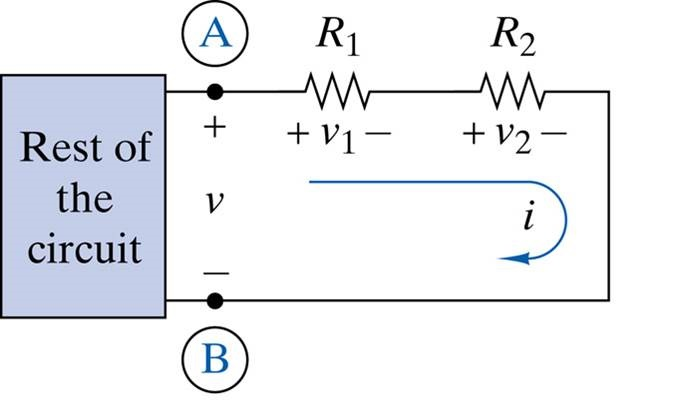
\includegraphics[width=0.5\textwidth]{Series_Resistors.jpg}
\caption{Series Resistors}
\label{fig: Series_Resistors}
\end{figure}

\subsection{Parallel}
What does it mean when we says devices are in parallel?

\soln{1.5in}{
\begin{enumerate}
\item If \textbf{two} and \textbf {or more} components share two common nodes, then those components are in parallel.
\item If two devices are connected to form a loop that contains only those two device, they are in parallel.
\item Parallel devices will all have the same voltage across them.
\end{enumerate}

In Figure \ref{fig: Parallel_Resistors}, devices 1,  2, and 3 are all  in parallel.  Notice that when taken pair-wise, you can form a loop with contains only 1 and 2, only 2 and 3, or only 1 and 3.
  Also you can see that all three device share two common nodes.  Last, it should be obvious that the voltage across all three devices is identical.
}

\begin{figure}[h t b]
\centering
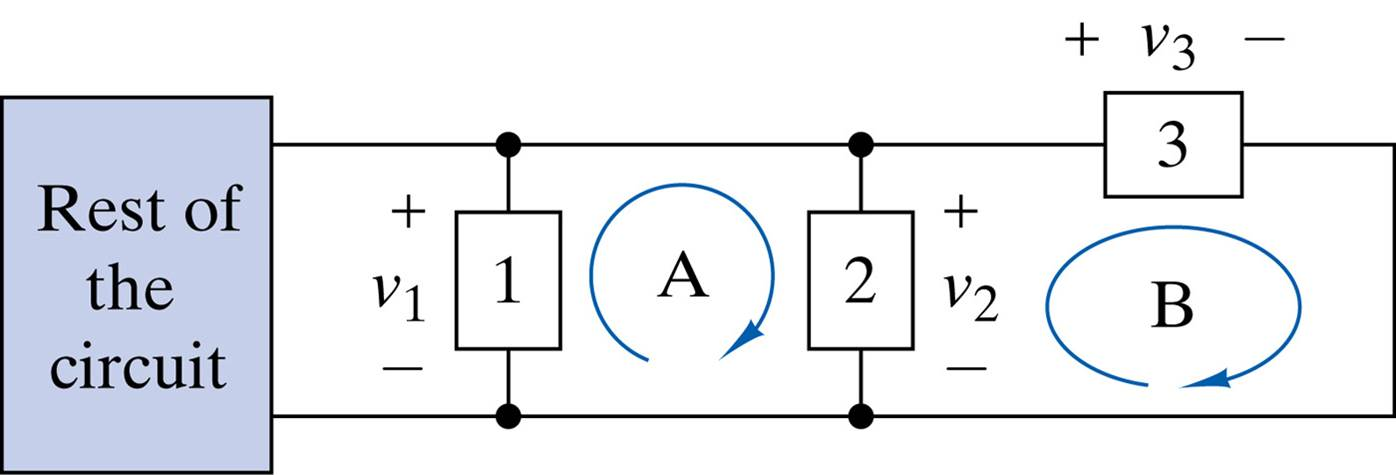
\includegraphics[width=0.5\textwidth]{Parallel_Resistors.jpg}
\caption{Parallel Resistors}
\label{fig: Parallel_Resistors}
\end{figure}

\section{Equivalent Circuits}
In this section we will discuss how to simplify circuits by combining resistors into equivalent resistance values and doing source transformation.  

\begin{description}
\item [Equivalent Circuits] are circuits that have identical voltage-current relationships at a given pair of terminals
\end{description}

\subsection{Equivalent Resistance, $R_{eq}$}
The first step in being able to analyze equivalent circuits is to be able to combine resistors into a total (or equivalent) resistance.  The method for combining parallel and series resistors is different and we will derive both here.

\subsubsection{Series $R_{eq}$}
To derive an equation for equivalent resistance in series circuites, lets look the circuit shown in Figure \ref{fig: Series_Resistors}. We can write a KVL equation for this circuit:

\soln{1in}{
\begin{equation}
v_{AB}-v_1-v_2 = 0
\end{equation}
}

We can define currents going into resistors $R_1$ and $R_2$ as $i_1$ and $i_2$ respectively.  Because of the Passive Sign Convention, the currents flow into the positive nodes of the resistors. Using that we can rewrite teh KVL equation as

\soln{1in}{
\begin{equation}
v_{AB}-i_1R_1-i_2R_2 = 0
\end{equation}
}

By examining the circuit (and from our definition of series resistors) we should see that $i_1=i_2=i$.  So again we can rewrite the KVL equation:

\soln{1in}{
\begin{eqnarray}
v_{AB}-iR_1-iR_2 &=& 0 \\
v_{AB}-i(R_1+R_2) &=& 0 \nonumber 
\end{eqnarray}
}

This final equation shows us that the series resistors can be modeled as a single resistor with an equivalent resistance of $R_1+R_2$.  This allows us to redraw the circuit in Figure \ref{fig: Series_Resistors} to a circuit with a single resistor; this new circuit is shown in Figure \ref{fig: SeriesReq}.

\begin{figure}[h t b]
\centering
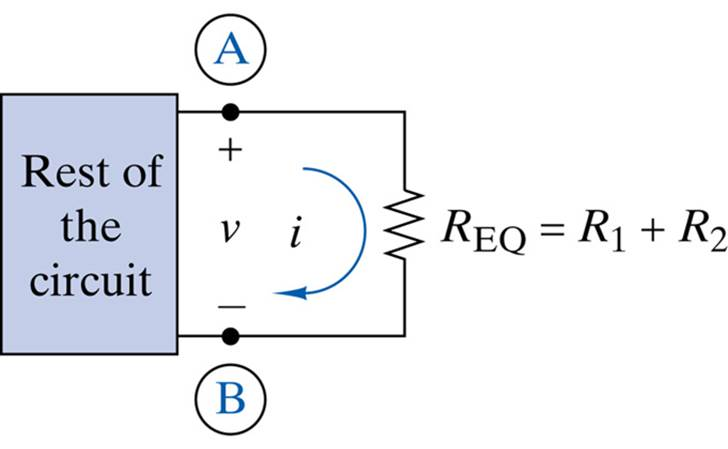
\includegraphics[width=0.5\textwidth]{SeriesReq.jpg}
\caption{Series Equivalent Resistance}
\label{fig: SeriesReq}
\end{figure}

So, for $k$ resistors in series:

\soln{1in}{
\begin{equation}
R_{eq}=\sum_{n=1}^k R_n
\end{equation}
}

$R_{eq}$ is always larger than any individual {\em series} resistor value.

\subsubsection{Parallel $R_{eq}$}
Before we derive the equation for parallel $R_{eq}$ we need to introduce the concept of conductance.  Conductance ($G$) is simply the inverse of resistance:
\begin{equation}
G=\frac{1}{R}
\end{equation}
We can now rewrite Ohm's law interms of conductances:
\soln{1in}{
\begin{equation}
i=vG
\end{equation}
}

Now that we have defined conductance, we can set off on deriving the equation for parallel equivalent resistance.

\begin{figure}[h t b]
\centering
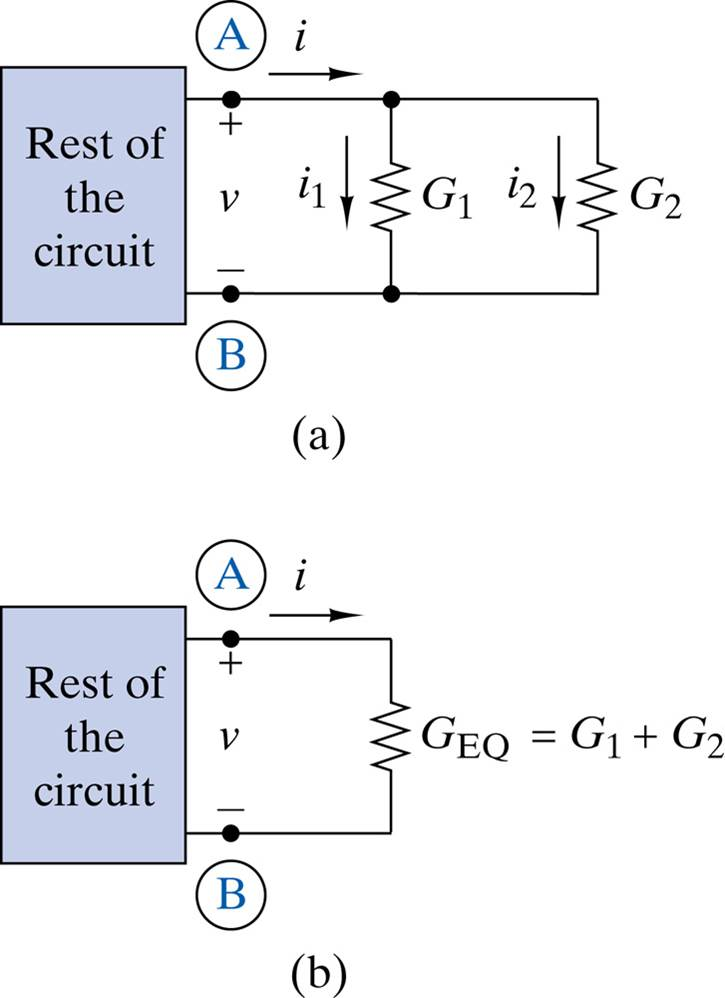
\includegraphics[width=0.5\textwidth]{ParallelReq.jpg}
\caption{(a) Circuit with two parallel resistors (b) Same circuit with one equivalent resistance}
\label{fig: ParallelReq}
\end{figure}

We start by examining the circuit shown in Figure \ref{fig: ParallelReq}(a). We can apply KCL at node A:
\soln{1in}{
\begin{equation}
i= i_1 + i_2
\end{equation}
}
We can now use Ohm's law (in terms of conductance) to replace all the currents above:
\soln{1in}{
\begin{equation}
vG_{eq}= vG_1 + vG_2
\end{equation}
}
where $G_{eq}$ is the circuits equivalent conductance.We can now factor and cancel the voltage ($v$), which gives:
\soln{1in}{
\begin{equation}
G_{eq}=G_1 +G_2
\end{equation}
}
But based on our definition of conductance, we have
\soln{1in}{
\begin{equation}
\frac{1}{R_{eq}}=\frac{1}{R_1} + \frac{1}{R_2}
\end{equation}
}
This is easily extend to any number of parallel resistors:
\soln{1in}{
\begin{equation}
\frac{1}{R_{eq}}=\sum_{n=1}^k\frac{1}{R_n}
\end{equation}
}

$R_{eq}$ is always smaller than any individual {\em parallel} resistor value.

\textbf{Cool Shortcut for 2 resistor case}....

\soln{1in}{
\begin{equation}
R_{eq}=\frac{R_1R_2}{R_1+R_2}
\end{equation}
}

If both resistors are equal resistance values, then this simplies to 

\soln{1in}{
\begin{equation}
R_{eq}=\frac{R}{2}
\end{equation}
}

\pagebreak

\subsubsection{Examples}
\textbf{Textbook Exercise 2-15 (p.39)}

Find the equivalent resistance between terminals A-C, B-D, A-D, \& B-C in Figure \ref{fig: Ex2_15}

\begin{figure}[h t b]
\centering
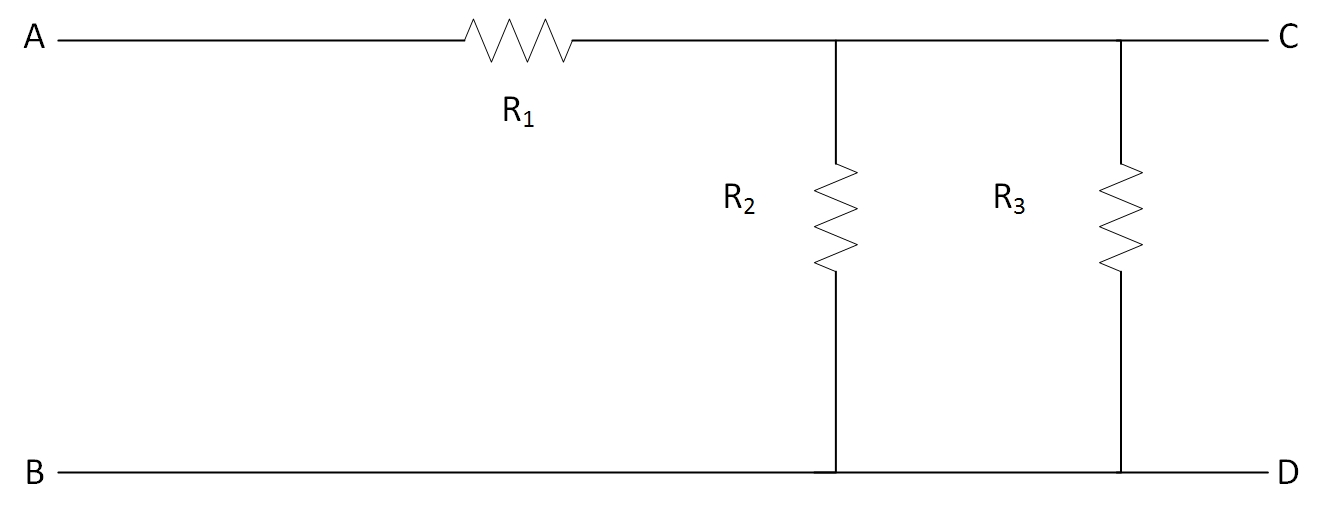
\includegraphics[width=0.5\textwidth]{Ex2_15.jpg}
\caption{Circuit for text book exercise 2-15}
\label{fig: Ex2_15}
\end{figure}

\soln{6in}{
\begin{figure}[h t b]
\centering
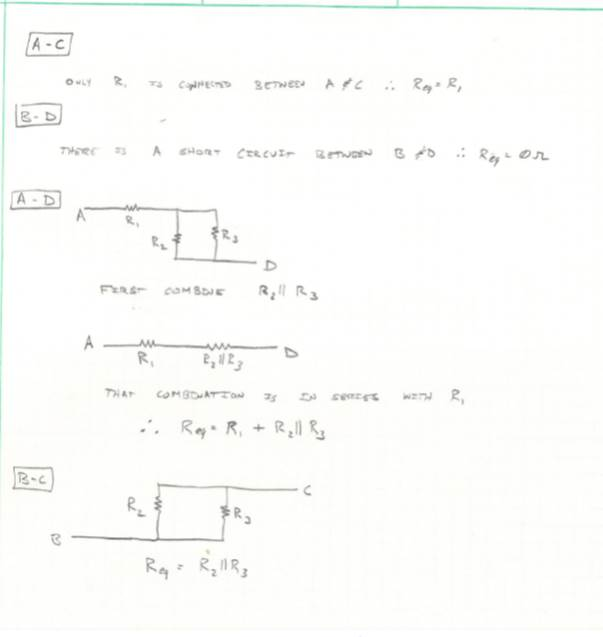
\includegraphics[width=0.7\textwidth]{Ex2_15soln.jpg}
\end{figure}
}

\clearpage

\textbf{Textbook Exercise 2-16 (p.39)}

Find the equivalent resistance between terminals A-B, A-C, A-D, B-C, B-D, \& C-D in Figure \ref{fig: Ex2_16}

\begin{figure}[h t b]
\centering
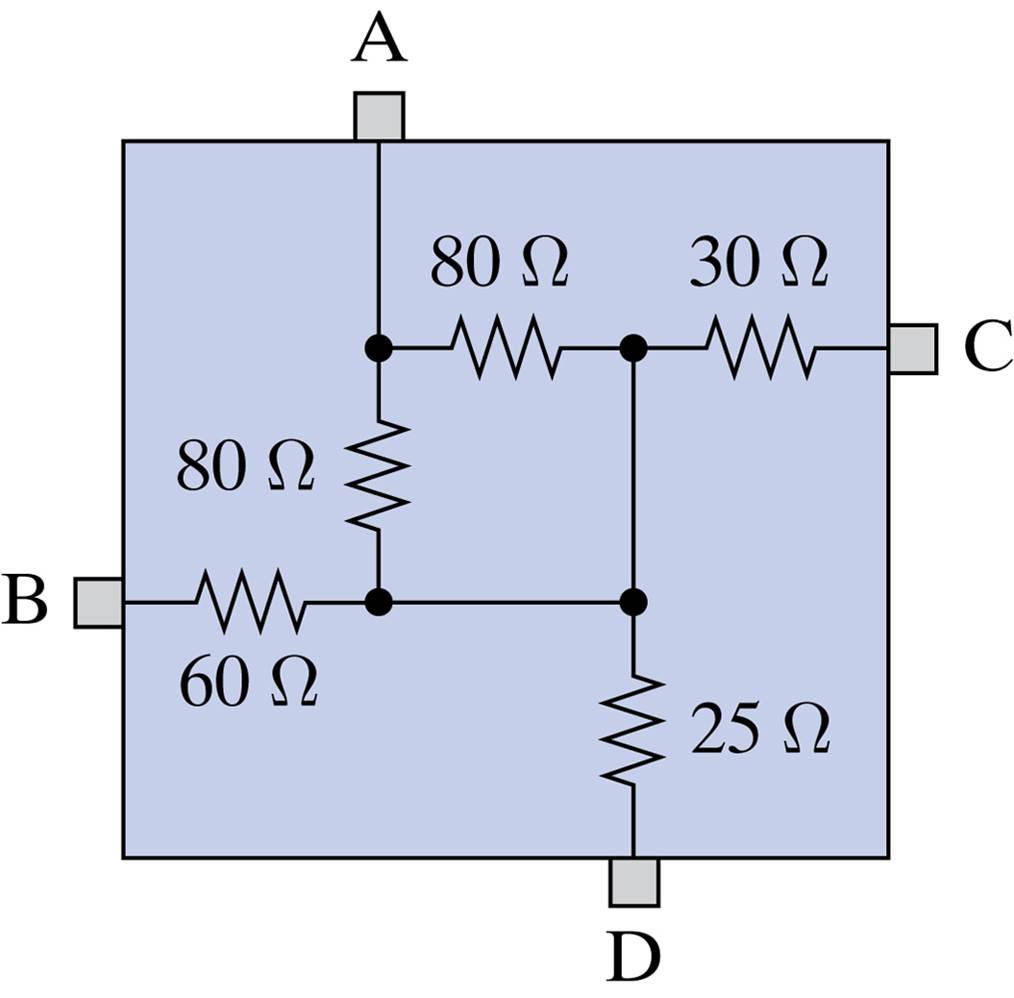
\includegraphics[width=0.5\textwidth]{Ex2_16.jpg}
\caption{Circuit for text book exercise 2-16}
\label{fig: Ex2_16}
\end{figure}

\soln{6in}{
\begin{figure}[h t b]
\centering
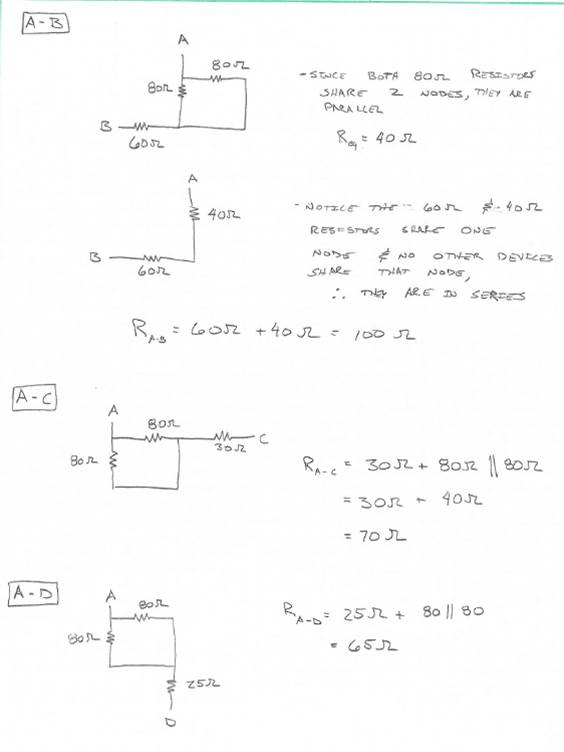
\includegraphics[width=0.9\textwidth]{Ex2_16solnA.jpg}
\end{figure}
}
\soln{6in}{
\begin{figure}[h t b]
\centering
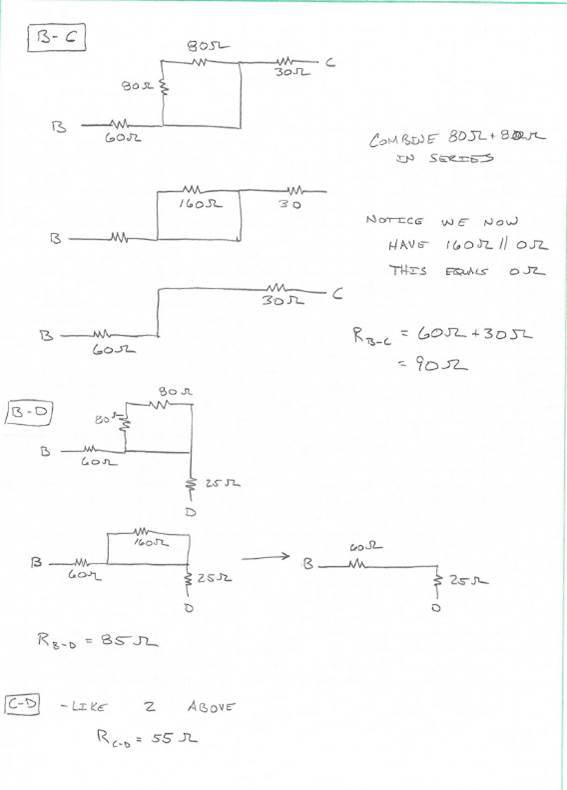
\includegraphics[width=0.9\textwidth]{Ex2_16solnB.jpg}
\end{figure}
}

\clearpage


\section{Review Questions}
\begin{questions}
\item When resistors are in parallel, $R_{eq}$ is bigger or smaller than the individual component resistances? 

\soln{1in}{Smaller}

\item What does $G$ represent? 

\soln{1in}{Conductance, $\frac{1}{R}$}

\item How do you know if resistors are in series? 

\soln{1in}{They share only one common node and no other devices share that node.  All the current from one device flows into the second device.}

\item True or False.... Resistors in series have the same voltage drop across them. 

\soln{1in}{True}

\newpage


\end{questions}

\end{document}


% Equation Array Example Code
%\begin
%{eqnarray}
%P_R &=& i_R^2R \nonumber \\
%P_R &=& (100\ mA)^2 \times 100\ \Omega \nonumber \\
%P_R &=& (100 \times 10^{-3}\ A)^2 \times 100\ \Omega \\
%P_R &=& 10000 \times 10^{-6}\ A^2  \times 100\ \Omega \nonumber \\
%P_R &=& 1\ W  \nonumber
%\end{eqnarray} 

% Figure Example Code
%\begin{figure} 
%\centering
%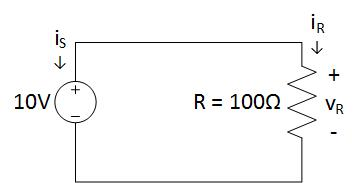
\includegraphics[width=0.5\textwidth]{OhmsLawExampleSolution.jpg}
%\caption{Ohm's Law example circuit}
%\label{fig: OhmsLawExampleSolution}
%\end{figure}

%Table Example Code
%\begin{table}[h]
%\centering
%\begin{tabular}{|l|c|c|}
%\hline
%Prefix & Abbreviation & Value \\
%\hline \hline
%Giga & $G$ & $10^9$ \\
%Mega & $M$ & $10^6$ \\
%Kilo & $k$ & $10^3$ \\
%\hline
%milli & $m$ & $10^{-3}$ \\
%micro & $\mu$ & $10^{-6}$ \\
%nano & $n$ & $10^{-9}$ \\
%pico & $p$ & $10^{-12}$ \\
%\hline
%\end{tabular}
%\caption{Engineering prefixes and values}
%\label{tab: Eng Prefixes}
%\end{table}
